% {\color{blue} 정돈되어있지 않아 정리 및 단어 통일화필요}

% {\color{blue} workload generate figure 필요한가? }

\section{Design Overview}
\label{sec:design_overview}

Figure~\ref{fig:system_overview}는 RL-SchedExt의 전체 System Architecture를 나타낸다.
RL-SchedExt는 Scheduling Policy를 학습하는 Offline Learning
단계와 학습된 Policy를 실제 CPU Scheduling에 적용하는
Runtime Inference 단계로 구성된다.
Offline Learning은 Linux Server에서 수행되며,
Runtime Inference는 Android Kernel 내부에서 수행된다.
이러한 구조는 Deadline 기반의 Reward를 확보하기 어려운
실제 Kernel 환경에서 학습을 수행할 필요 없이,
학습된 Scheduling Policy를 적용할 수 있도록 한다.

\begin{figure}[H]
    \centering
    \IfFileExists{Figures/System_overview.png}{%
        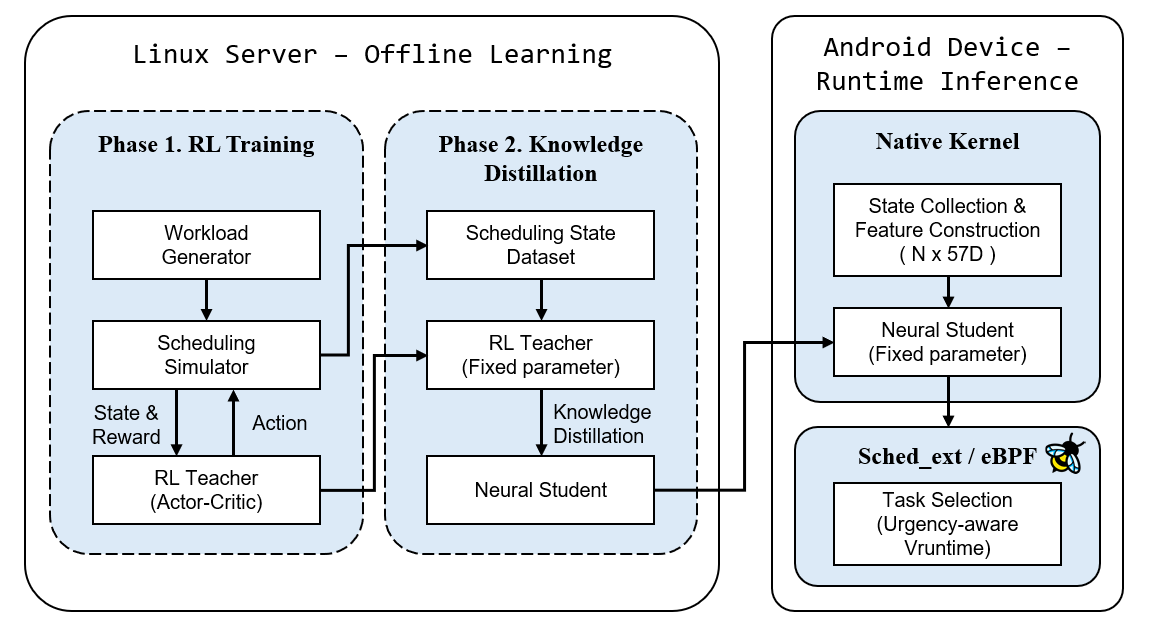
\includegraphics[width=\linewidth,keepaspectratio]{Figures/System_overview.png}%
    }{%
        \fbox{\parbox[c][0.50\linewidth][c]{0.94\linewidth}{%
            \centering System Overview Figure\\
            Upload \texttt{Figures/System\_overview.png} to display the figure.}}%
    }
    \caption{Overall architecture of RL-SchedExt.
    Offline learning consists of RL Teacher training and
    teacher--student knowledge distillation on a Linux server.
    The trained Neural Student is deployed to the Android kernel,
    where its inference results are used for eBPF-based task selection.}
    \label{fig:system_overview}
\end{figure}

\paragraph{Offline Learning.}
Figure~\ref{fig:system_overview}의 Linux Server에서는 Offline Learning을 두 단계로 수행한다.
Phase 1 (RL Teacher Training)에서는 Workload Generator에서 생성한 Workload를 기반으로 Scheduling Simulator를 구성하고, Simulator와의 상호작용을 통해 RL Teacher의 Scheduling Policy를 학습한다.
Simulator는 Kernel에서 관측 가능한 State와 Scheduling Decision에 따른 Deadline-oriented Reward를 제공한다.
Phase 2 (Knowledge Distillation)에서는 Scheduling State Dataset을 학습이 완료된 RL Teacher와 Neural Student에 입력하고, Teacher--Student Knowledge Distillation을 통해 경량 Neural Student를 학습시킨다.
학습된 Neural Student는 INT8 Quantization을 거쳐 Android Kernel에 배포된다.

\paragraph{Runtime Inference.}
Figure~\ref{fig:system_overview}의 Android Device에서는 학습된 Neural Student를 이용하여 Runtime Inference를 수행한다.
Native Kernel은 Runtime State Collection을 통해 Scheduling Event마다 Runtime History를 갱신하고, Task Selection 시점에 Runnable Task Set의 각 Task에 대해 57차원의 State를 구성한다.
Native Kernel의 Neural Student가 Runnable Task Set 내 각 Task의 Learned Vruntime Adjustment를 계산하면, sched\_ext의 eBPF Scheduling Program은 Urgency-aware Vruntime을 기준으로 다음 Task를 선택한다.
Native Kernel은 선택 결과를 검증하여 실제 Task Dispatch에 반영한다. 이러한 구체적인 Runtime 구현 방법은 다음 Chapter에서 설명한다.

RL-SchedExt의 학습 대상은 하나의 CPU에서 경쟁하는 Runnable Task Set의 실행 순서이며, Time Slice와 Preemption은 CFS 방식의 Scheduling Mechanism을 기반으로 처리한다.
Runtime에서는 RL Teacher, Scheduling Simulator 및 Reward 계산이 필요하지 않으며, 학습된 Neural Student의 Weight와 Bias를 고정하여 사용한다.

\section{Simulation-based Learning Environment}
%- Linux Server에서 수행되는 것 설명
%- Simulator 기반 학습 선택한 이유 및 장점
%- 실제 CPU에서의 task execusion과 simulation에서의 차이

실제 Android Kernel에서는 Application Request의 Deadline과 Scheduling Decision의 결과를 학습에 필요한 Reward로 확보하기 어렵다.
또한 실제 Device에서 다양한 Scheduling Policy를 반복적으로 평가하는 데에는 실행 환경의 변동성과 실험 비용이라는 제약이 존재한다.
따라서 RL-SchedExt는 Linux Server에서 가상 시간 기반의 Scheduling Simulator를 이용하여 다양한 Workload와 Scheduling Decision에 따른 실행 결과를 생성한다.
이를 통해 Kernel에서 관측 가능한 State와 Deadline-oriented Reward 사이의 관계를 학습할 수 있는 환경을 구성한다.

\subsection{Workload Modeling}
%- Task 종류 설명 (CPU-bound, Periodic,...) 및 왜 해당 task 종류로 classification했는지
%- Randomized Workload Generation 및 json file output.
실제 시스템에서는 서로 다른 실행 특성과 의존 관계를 가진
Task들이 제한된 CPU 자원을 공유한다.
각 Task는 서로 다른 CPU 실행 특성과 Wakeup Pattern을 가지며,
일부 Task는 다른 Task의 실행 결과나 공유 자원의 상태에 따라
실행 가능 여부가 결정된다.

RL-SchedExt는 이러한 Scheduling 상황을 모사하기 위해
다음과 같은 Task의 실행 특성 및 의존 관계를 모델링한다.

\begin{itemize}
    \item \textbf{CPU-bound:}
    상대적으로 긴 CPU Demand를 가지며 지속적으로
    CPU 자원을 요구하는 실행 특성.

    \item \textbf{I/O-bound:}
    CPU Execution과 I/O Blocking을 반복하며
    빈번한 Sleep 및 Wakeup이 발생하는 실행 특성.

    \item \textbf{Periodic Wakeup:}
    일정한 시간 간격으로 새로운 작업이 Release되는
    실행 특성.

    \item \textbf{Random Burst:}
    불규칙한 시점에 다양한 크기의 CPU Demand가
    발생하는 실행 특성.

    \item \textbf{Chain Dependency:}
    선행 Task의 실행 완료에 따라 후속 Task가 실행 가능한
    상태로 전환되는 순차적 의존 관계.

    \item \textbf{Lock Dependency:}
    공유 자원을 보유한 Task의 Lock Release에 따라
    다른 Task의 실행 가능 여부가 결정되는 의존 관계.
\end{itemize}

Scheduling Simulator는 Task와 Request를 구분하여 관리한다.
Task는 Scheduling Weight, Vruntime, Wakeup Pattern 및 실행 상태를 가지며,
Request는 Arrival Time과 Deadline Budget을 가진다.
Request를 처리하기 위한 CPU Demand는 하나 이상의 Task에 할당되는
실행 작업으로 표현되며, 실행 특성에 따라 Blocking 조건과
Task 간 Dependency가 추가적으로 정의된다.
Absolute Deadline은 Request의 Arrival Time과 Deadline Budget으로부터 결정된다.
Simulator는 이러한 실행 특성과 의존 관계를 조합하여 하나의 Workload를 구성한다.
학습 과정에서는 Task의 수, CPU Demand, Request Arrival Pattern,
Deadline Budget 및 Dependency 등을 Randomization하여
다양한 CPU 경쟁 상황을 생성한다.
이러한 Workload Modeling을 통해 RL Policy가 특정
Application의 실행 패턴에 overfitting되지 않고,
다양한 Task 특성과 의존 관계에서 발생하는 Scheduling
Dynamics를 학습하도록 한다.

\subsection{Modeling CFS Scheduling Dynamics}

Scheduling Simulator는 Linux CFS의 주요 Scheduling
Dynamics를 기반으로 가상의 CPU와 Task의 실행 상태를
관리한다.
실제 Process 또는 Thread를 CPU에서 실행하는 대신,
각 Task를 Scheduling Entity로 표현하고 Simulation Clock을
진행시키면서 Scheduling State를 갱신한다.

각 Scheduling Entity는 현재 처리 중인 실행 작업의 Remaining CPU Demand,
Remaining Time Slice, Vruntime, Scheduling Weight
및 Task State 등의 정보를 유지한다.

Task $i$의 Remaining CPU Demand를 $D_i(t)$,
Remaining Time Slice를 $S_i(t)$,
Vruntime을 $V_i(t)$라고 정의한다.
Task $i$가 $\delta t$만큼 CPU 시간을 할당받으면,
Simulator는 해당 Task가 동일한 양의 CPU 시간을
사용한 것으로 간주한다.

이에 따라 Remaining CPU Demand와 Remaining Time Slice는
다음과 같이 갱신된다.

\begin{equation}
    D_i(t+\delta t)
    =
    \max(0,D_i(t)-\delta t)
\end{equation}
\begin{equation}
    S_i(t+\delta t)
    =
    \max(0,S_i(t)-\delta t)
\end{equation}

Vruntime은 Background에서 설명한 CFS의
Scheduling Weight 기반 CPU Accounting 원리를 적용하여
다음과 같이 갱신된다.

\begin{equation}
    V_i(t+\delta t) = V_i(t)+\delta t\frac{w_0}{w_i}
\end{equation}

여기서 $w_i$는 Task $i$의 Scheduling Weight이며, $w_0$는 Nice-0 Scheduling Weight이다.

Simulation Clock이 진행됨에 따라 Simulator는
Task Release, Wakeup, Blocking, Task Completion 및
Time Slice Expiration 등의 Scheduling Event를 처리한다.
Remaining CPU Demand($D_i(t)$)가 0에 도달하면 해당 실행 작업이
완료된 것으로 처리하며, Request Completion은 해당 Request에
필요한 실행 작업들이 완료되었는지를 기준으로 판단한다.
Remaining Time Slice($S_i(t)$)가 소진되거나
Preemption 조건이 충족되면 새로운 Scheduling Decision을
수행할 수 있다.

I/O Blocking이나 Lock Dependency가 발생한 Task는
Runnable Task Set에서 제외되며,
I/O Completion, Lock Release 또는 선행 Task의 완료 등
실행 가능 조건이 충족되면 Runnable 상태로 전환된다.

CFS를 모사하는 기본적인 Task Selection은
Runnable Task Set $\mathcal{R}(t)$에 대해 다음과 같이
표현할 수 있다.

\begin{equation}
    i^*_{\mathrm{CFS}}
    =
    \arg\min_{i \in \mathcal{R}(t)} V_i(t)
\end{equation}

이러한 Scheduling Dynamics를 기반으로 Simulator는
Task의 실행 순서에 따른 CPU 자원 경쟁, Task 간 의존 관계
및 Completion Time의 변화를 수치적으로 모사한다.

\subsection{Simulation Scope and Abstraction}

Scheduling Simulator는 실제 CPU의 Cache, Memory Stall,
Instruction Execution 등의 Microarchitectural Behavior를
직접적으로 모사하지 않으므로 실제 Device와의
Simulation-to-Reality Gap이 존재할 수 있다.
그러나 RL-SchedExt의 학습 목적은 Hardware 수준의
실행 특성을 정확하게 재현하는 것이 아니라,
Scheduling Decision이 Workload의 실행 결과에 미치는
영향을 학습하는 것이다.
따라서 Simulator는 Hardware-specific Behavior를 추상화하고,
Task의 실행 상태, CPU 자원 경쟁 및 Task 간 의존 관계를
중심으로 Scheduling Environment를 구성한다.
이를 통해 RL Teacher가 다양한 Scheduling Context에서
Task의 실행 순서에 따른 Deadline Miss Count 및 Request Completion Latency의
변화 경향을 학습할 수 있도록 설계하였다.

\section{Reinforcement Learning Formulation}
% - CPU Scheduling의 순차적 의사결정 문제 정의
% - Deadline을 직접 관측할 수 없는 문제
CPU Scheduling은 현재 실행할 Task의 선택이 이후의
Task State와 CPU 경쟁 상황에 영향을 미치는
순차적 의사결정 문제이다.
특히 Task 간 의존 관계가 존재하는 경우,
특정 Task의 실행 순서는 해당 Task가 처리하는 Request의
Completion Time뿐만 아니라 의존 관계에 있는 다른 Task의 실행 가능 시점과
관련 Request의 Deadline 충족 여부에도 영향을 미친다.

그러나 실제 Kernel에서는 Application Request의 Deadline과
미래 CPU Demand를 직접 관측하기 어렵다.
따라서 RL-SchedExt는 Scheduling Simulator에서 제공하는
Deadline 기반 Reward를 이용하여,
Kernel에서 관측 가능한 Runtime State와
Scheduling Decision 사이의 관계를 학습한다.
이를 위해 CPU Scheduling 문제를 State, Action 및
Reward로 구성된 Reinforcement Learning 문제로 정의한다.

\subsection{State: Context-aware Representation}
% - Kernel에서 관측 가능한 Runtime Feature
% - 13D Task Feature 및 6D Global Feature
% - 38D Derived Context Feature
% - 57D State 구성 및 선정 이유
% - Table: State Feature Definition (자세히 설명하는거는 19D만하고 38D 는 derived했다고 표현.
RL-SchedExt는 실제 Kernel에서 수집할 수 있는 Runtime Feature를 기반으로 Task의 실행 특성과 현재 Scheduling Context를 표현한다.
Application Request의 실제 Deadline, Remaining CPU Demand 및 미래 Wakeup 정보는 Runtime State에 포함하지 않는다.

State의 Base Feature는 개별 Task의 실행 특성을 나타내는 13개의
Task Feature와 현재 CPU의 Scheduling 환경을 나타내는 6개의 Global Feature로 구성된다.
Table~\ref{tab:state_features}는 각 Feature의 정의를 보여준다.
여기서 Exponentially Weighted Moving Average (EWMA)는 실행 이력의
이동 평균을, Coefficient of Variation (CV)은 Wakeup Interval의 변동성을
나타낸다.

\begin{table}[t]
    \centering
    \scriptsize
    \setlength{\tabcolsep}{3pt}
    \renewcommand{\arraystretch}{1.15}
    \begin{tabularx}{\linewidth}{|>{\centering\arraybackslash}p{0.08\linewidth}|>{\raggedright\arraybackslash}p{0.32\linewidth}|>{\raggedright\arraybackslash}X|}
        \hline
        \textbf{Dim.} & \textbf{Feature} & \textbf{Description} \\ \hline
        \multicolumn{3}{|c|}{\textbf{Task Features (13D)}} \\ \hline
        1 & Vruntime
          & Virtual Runtime expressed relative to a common reference \\ \hline
        1 & Log2 Weight
          & Log-scaled relative scheduling weight \\ \hline
        1 & CPU Utilization
          & EWMA of CPU execution ratio \\ \hline
        1 & Runnable Ratio
          & EWMA of runnable time ratio \\ \hline
        1 & Current Wait
          & Current runnable waiting time \\ \hline
        1 & Wait EWMA
          & Historical average waiting time \\ \hline
        1 & Wakeup Rate
          & Wakeup frequency \\ \hline
        1 & Time Since Last Run
          & Elapsed time since last execution \\ \hline
        1 & Preemption Rate
          & Preemption frequency \\ \hline
        1 & Sleep/Block Rate
          & Sleep or blocking frequency \\ \hline
        1 & Time Since Quiescent
          & Time since last inactive State \\ \hline
        1 & Wakeup CV
          & Variability of wakeup intervals \\ \hline
        1 & Service Debt
          & CPU service deficit relative to fair share \\ \hline
        \multicolumn{3}{|c|}{\textbf{Global Features (6D)}} \\ \hline
        1 & Runnable Count
          & Number of runnable tasks \\ \hline
        1 & Mean Wait
          & Mean runnable waiting time \\ \hline
        1 & Max Wait
          & Maximum runnable waiting time \\ \hline
        1 & Vruntime Spread
          & Range of runnable Task vruntimes \\ \hline
        1 & CPU Utilization
          & EWMA of CPU utilization \\ \hline
        1 & Context Switch Rate
          & Context switch frequency \\ \hline
        \multicolumn{3}{|c|}{\textbf{Derived Context Features (38D)}} \\ \hline
        5 & Relative Rank
          & Relative feature ranks among runnable tasks \\ \hline
        5 & Relative Difference
          & Feature gaps relative to other tasks
            and aggregate values \\ \hline
        6 & Runnable Task Set Statistics
          & Aggregate statistics of runnable tasks \\ \hline
        6 & Other Task Statistics
          & Statistics excluding the current Task \\ \hline
        5 & First CFS Task
          & Features of the minimum-Vruntime Task \\ \hline
        5 & First CFS Task Difference
          & Feature differences from the first CFS Task \\ \hline
        3 & Second CFS Task
          & Features of the second minimum-Vruntime Task \\ \hline
        3 & Second CFS Task Difference
          & Feature differences from the second CFS Task \\ \hline
        \textbf{57} & \multicolumn{2}{|c|}{\textbf{Total}} \\ \hline
    \end{tabularx}
    \caption{State representation of RL-SchedExt.}
    \label{tab:state_features}
\end{table}

Task Feature는 Task의 CPU 사용 이력, Wakeup Pattern, Runnable Waiting Time 및 CPU 자원 할당 상태를 표현한다.
이를 통해 직접 관측할 수 없는 Task의 실행 특성을
과거 및 현재의 Runtime Behavior로부터 간접적으로
파악할 수 있도록 한다.

Global Feature는 현재 Runnable Task의 수,
대기 시간 및 CPU Utilization 등을 포함하여,
개별 Task의 실행 특성만으로는 표현하기 어려운
CPU 자원 경쟁 상황을 나타낸다.

그러나 동일한 Task Feature를 가지더라도
현재 경쟁하는 다른 Task의 실행 특성에 따라
해당 Task의 Scheduling Urgency는 달라질 수 있다.
예를 들어 동일한 Wakeup Rate를 가진 Task라도
경쟁 Task 대부분이 CPU-bound인 경우와
빈번하게 Wakeup하는 Task인 경우에는
해당 Task를 우선적으로 실행하는 것이 전체 Workload에
미치는 영향이 다를 수 있다.

이러한 상대적인 Scheduling Context를 표현하기 위해
RL-SchedExt는 Base Feature로부터 38개의
Derived Context Feature를 추가적으로 구성한다.
Table~\ref{tab:state_features}에서 나타낸 것과 같이,
Derived Context Feature는 Runnable Task Set의
통계적 특성, 현재 Task의 상대적인 Feature 순위 및
CFS의 Vruntime 기준 첫 번째와 두 번째 실행 우선순위를
가지는 Task와의 비교 정보를 포함한다.
이를 통해 개별 Task의 실행 특성뿐만 아니라
기존 CFS의 Task Ordering와 현재 Task 간의
상대적인 관계를 Policy의 입력으로 제공한다.

최종적으로 Task $i$의 State는 다음과 같이 정의된다.

\begin{equation}
    \mathbf{s}_i = \left[\underbrace{\mathbf{x}_i}_{\text{13D Task}},\ \underbrace{\mathbf{g}}_{\text{6D Global}},\ \underbrace{g_{\mathrm{ctx}}(\mathbf{x}_i,\mathbf{g},\mathcal{R}_k)}_{\text{38D Derived}}\right] \in \mathbb{R}^{57}
    \label{eq:state_representation}
\end{equation}

여기서 $\mathcal{R}_k=\mathcal{R}(t_k)$는 실제 시각 $t_k$에서
Scheduling Decision Step $k$에 사용되는 Runnable Task Set이며,
$g_{\mathrm{ctx}}$는 Context Feature Extraction Function이다.
Scheduling State $S_k$는 해당 Runnable Task Set에 포함된 각 Task의
57차원 State를 Task Index에 대응시킨 집합 표현이다.

\begin{equation}
    S_k = (\mathbf{s}_i)_{i\in\mathcal{R}_k}
    \label{eq:scheduling_state}
\end{equation}

이후 실제 시각은 $t$, Scheduling Decision Step은 $k$로 구분한다.
실제 구현에서 Runnable Task Set이 지원 범위를 초과할 경우에는
Chapter~4에서 설명하는 Fallback Selection Path를 사용한다.

따라서 Neural Student의 57차원 State는 57개의 독립적인
Kernel 정보를 수집하는 것이 아니라,
19개의 Base Feature와 이들로부터 계산된 38개의
Derived Context Feature로 구성된다.
이러한 State Representation은 개별 Task의 실행 특성과
Task 간 상대적인 관계를 함께 표현함으로써,
현재 Scheduling Context에 따른 Learned Vruntime Adjustment를
학습할 수 있도록 설계되었다.


\subsection{Action: Urgency-aware Task Ordering}
% - RL Action 정의
% - Learned Vruntime Adjustment
% - Urgency-aware Vruntime 계산 공식 : Vruntime + Learned Vruntime Adjustment
% - Task Selection 공식 : min(Urgency-aware Vruntime) 

RL-SchedExt의 Action은 현재 Runnable Task Set에서
다음 실행할 Task를 선택하는 것으로 정의된다.
이를 위해 Policy는 각 Task의 State와 Scheduling Context를
기반으로 Learned Vruntime Adjustment($\Delta V_i$)를 계산한다.

\begin{equation}
    \Delta V_i = f_{\theta}(\mathbf{s}_i,\mathcal{R}_k)
    \label{eq:learned_adjustment}
\end{equation}

여기서 $f_{\theta}$는 학습된 Scheduling Policy, $\mathbf{s}_i$는 Task $i$의 State,
$\mathcal{R}_k$는 Scheduling Decision Step $k$의 Runnable Task Set이다.

기존 Vruntime에 Learned Vruntime Adjustment를
반영한 값을 Urgency-aware Vruntime으로 정의한다.

\begin{equation}
    \underbrace{V_i^{\mathrm{urgency}}}
        _{\text{Urgency-aware Vruntime}}
    =
    \underbrace{V_i}
        _{\text{Vruntime}}
    +
    \underbrace{\Delta V_i}
        _{\text{Learned Vruntime Adjustment}}
    \label{eq:urgency_aware_vruntime}
\end{equation}

Learned Vruntime Adjustment는 Task의 Scheduling Urgency를
기존 Fairness 기반 Task Ordering에 반영하기 위한 조정값이다.
다른 조건이 동일할 때 음의 Adjustment는 Task의 Scheduling Priority를
높이며, 양의 Adjustment는 Scheduling Priority를 낮춘다.

Runtime Inference에서는 Runnable Task Set $\mathcal{R}_k$ 내에서
가장 작은 Urgency-aware Vruntime을 가지는 Task를
다음 실행 대상으로 선택한다.

\begin{equation}
    a_k =
    \underset{i\in\mathcal{R}_k}{\arg\min}
    V_i^{\mathrm{urgency}}
    \label{eq:task_selection}
\end{equation}

Learned Vruntime Adjustment는 기존 Vruntime의
Accounting 값을 변경하지 않으며,
Task Selection에만 사용된다.
본 논문에서는 Scheduling 원리의 설명을 위해 개념적인 Vruntime $V_i$를
사용한다. 실제 구현에서는 Runnable Task Set 전체에 공통된 기준 Vruntime을
차감한 값을 사용하지만, 동일한 기준값을 차감하므로 Task Ordering은
변하지 않는다.


\begin{table}[t]
    \centering
    \small
    \setlength{\tabcolsep}{3pt}
    \renewcommand{\arraystretch}{1.15}
    \begin{tabularx}{\linewidth}{|>{\centering\arraybackslash}p{0.18\linewidth}|>{\centering\arraybackslash}X|>{\centering\arraybackslash}p{0.16\linewidth}|}
        \hline
        \textbf{Symbol} & \textbf{Reward Component} & \textbf{Reward Weight} \\ \hline
        \multicolumn{3}{|c|}{
            \textbf{Primary Reward Components}} \\ \hline
        $R_k^{\mathrm{req}}$
            & Completed Request Reward & $+1.0$ \\ \hline
        $M_j$
            & Deadline Miss & $-3.0$ \\ \hline
        $O_j$
            & Deadline Overrun & $-1.5$ \\ \hline
        $L_j$
            & Request Completion Latency & $-0.3$ \\ \hline
        \multicolumn{3}{|c|}{
            \textbf{Auxiliary Reward Components}} \\ \hline
        $B_k$
            & Background CPU Service (ms) & $+0.12$ \\ \hline
        $W_k$
            & Runnable Waiting Time (ms) & $-0.015$ \\ \hline
        $U_k$
            & Wakeup-to-run Latency (ms) & $-0.04$ \\ \hline
        $H_k$
            & Context Switch Overhead (ms) & $-0.12$ \\ \hline
        $N_k^{\mathrm{switch}}$
            & Context Switch Count & $-0.003$ \\ \hline
        $R_k^{\mathrm{end}}$
            & Unfinished Work Penalty & $+1.0$ \\ \hline
    \end{tabularx}
    \caption{Reward components and their weights.}
    \label{tab:reward_components}
\end{table}

\subsection{Reward: Deadline-oriented Optimization}
% - Reward function 전체 공식 설명
% - Deadline Miss, Deadline Overrun, Request Completion Latency 구성요소 설명 하면서 Deadline miss만 최적화 하면 안되는 이유 간단 설명.
% - Reward Component별 Weight 및 Normalization

RL-SchedExt는 Deadline Miss, Deadline Overrun 및
Request Completion Latency를 주요 Optimization Objective로 설정한다.
또한 Background CPU Service, Runnable Waiting Time,
Wakeup-to-run Latency 및 Scheduling Overhead를 고려하여
Step Reward를 다음과 같이 정의한다.

\begin{equation}
    r_k = R_k^{\mathrm{req}} + \lambda_b B_k - \lambda_w W_k - \lambda_u U_k - \lambda_o H_k - \lambda_s N_k^{\mathrm{switch}} + R_k^{\mathrm{end}}
    \label{eq:total_reward}
\end{equation}

Table~\ref{tab:reward_components}는 전체 Reward Function의
각 Component와 적용되는 Reward Weight를 나타낸다.

Request Reward는 Application Request가 완료되는 시점에
해당 Request의 실행 결과를 기반으로 계산된다.
Background에서 정의한 성능 지표를 이용하여
Request $j$에 대한 Reward를 다음과 같이 정의한다.

\begin{equation}
    R_j =
    -\underbrace{\alpha M_j}_{\text{Deadline Miss}}
    -\underbrace{\beta O_j}_{\text{Deadline Overrun}}
    -\underbrace{\gamma L_j}_{\text{Request Completion Latency}}
    \label{eq:request_reward}
\end{equation}

Scheduling Decision Step $k$부터 다음 Step까지
완료된 Request의 집합을 $\mathcal{J}_k$라고 하면,
해당 구간의 Request Reward는 다음과 같이 계산된다.

\begin{equation}
    R_k^{\mathrm{req}}
    =
    \sum_{j\in\mathcal{J}_k}R_j
    \label{eq:request_reward_sum}
\end{equation}

% \clearpage
\section{Neural Policy Learning and Distillation}
% - Scheduling Performance와 Inference Cost의 Trade-off
% - Teacher-Student 구조의 설계 목적
% - Figure RL Teacher 와 Student network 구조그리기
Figure~\ref{fig:teacher_student_architecture}는 RL Teacher Training과 Knowledge Distillation으로 구성된 두 단계의 Offline Learning 과정을 나타낸다.

\begin{figure}[H]
    \centering

    \begin{subfigure}[b]{0.49\linewidth}
        \centering
        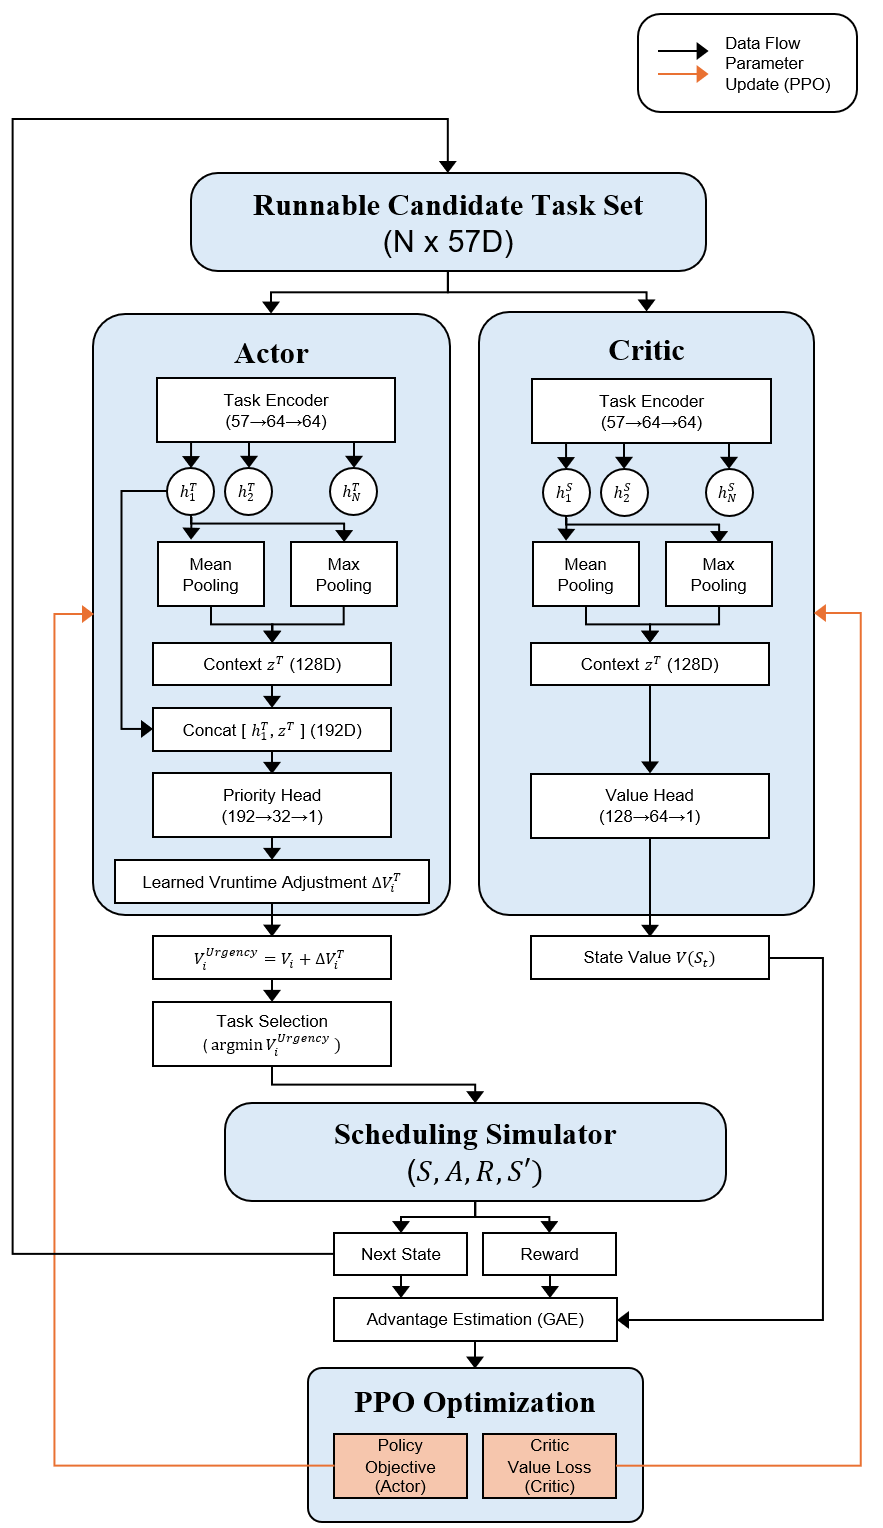
\includegraphics[
            width=\linewidth,
            keepaspectratio
        ]{Figures/ActorCritic.png}
        \caption{Phase 1: RL Teacher Training}
        \label{fig:actor_critic}
    \end{subfigure}
    % \hfill
    \hspace{1pt}%
    \begin{subfigure}[b]{0.49\linewidth}
        \centering
        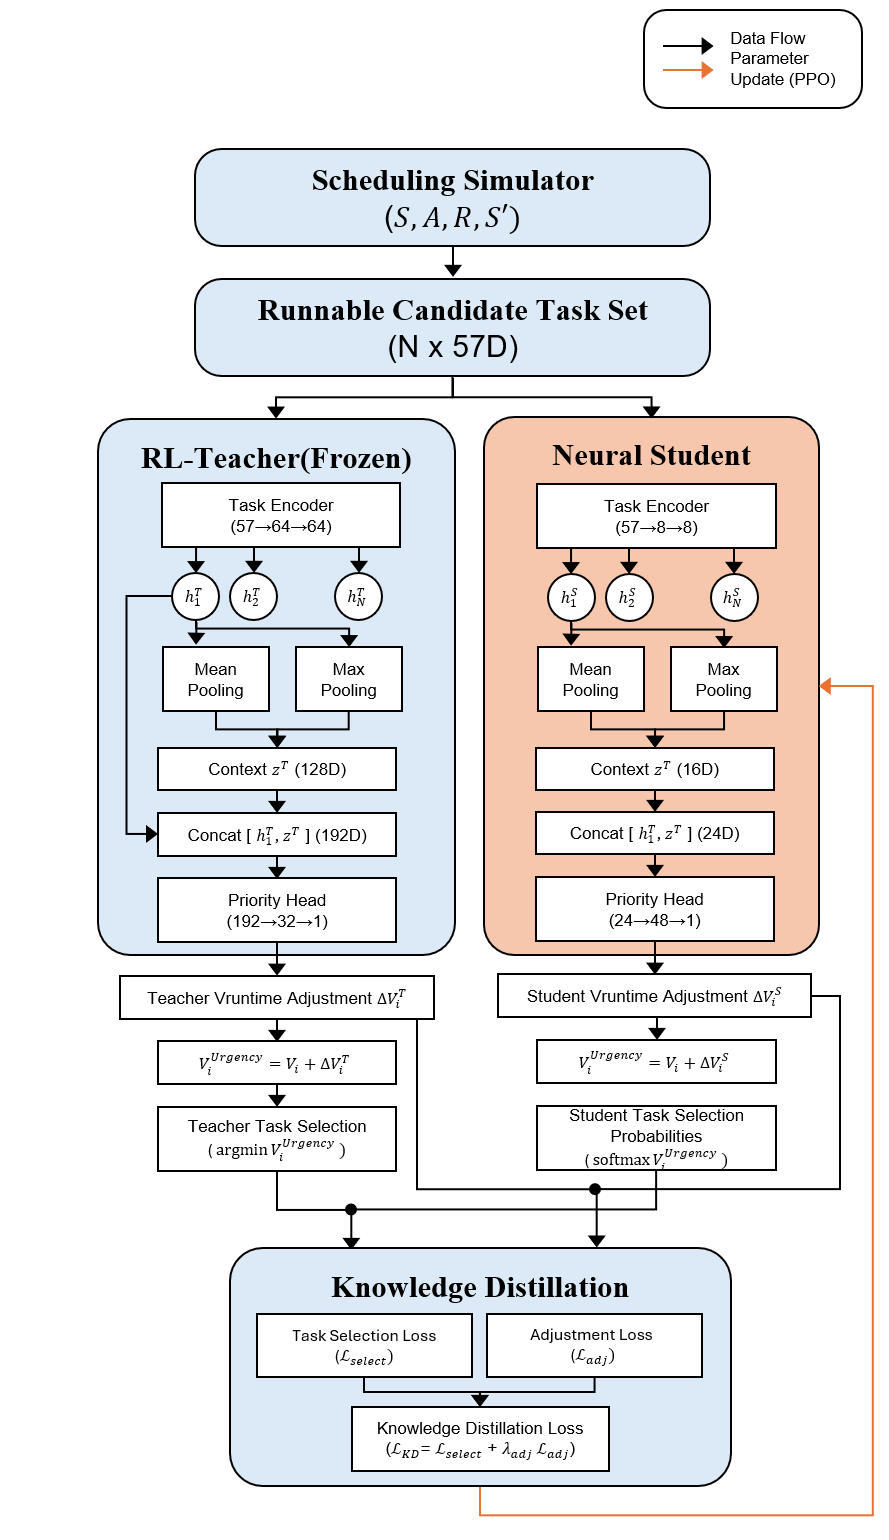
\includegraphics[
            width=\linewidth,
            keepaspectratio
        ]{Figures/TeacherStudent.png}
        \caption{Phase 2: Knowledge Distillation}
        \label{fig:teacher_student}
    \end{subfigure}

    \caption{RL-SchedExt의 2단계 Offline Learning Framework.
    Phase 1 (RL Teacher Training)에서는 RL Teacher가 Scheduling Simulator와의
    상호작용을 통해 문맥 의존적(Context-dependent)
    Scheduling Policy를 학습한다.
    Phase 2 (Knowledge Distillation)에서는 RL Teacher의 Weight와 Bias를 고정한 상태에서
    지식 증류(Knowledge Distillation)를 통해 학습된 Policy를
    경량 Neural Student에 전달한다.}
    \label{fig:teacher_student_architecture}
\end{figure}

\subsection{RL Teacher Policy}
% - Teacher Neural Network Architecture
% - Actor-Critic Architecture
% - Context Encoding 및 Policy Output
% - PPO 기반 Policy Optimization
RL Teacher Training에서는 다양한 Scheduling Context에서
Deadline-oriented Scheduling Policy를 학습하기 위해
DeepSets 기반의 Actor--Critic Architecture를 사용한다.
Figure~\ref{fig:teacher_student_architecture}(\subref{fig:actor_critic})는 RL Teacher의
Network Architecture와 Proximal Policy Optimization (PPO) 기반의 학습 과정을 나타낸다.

\paragraph{Actor Network Architecture.}
Actor는 현재 Runnable Task Set을 입력받아
각 Task의 Learned Vruntime Adjustment를 계산한다.
각 Task의 57차원 State는 공유된 Task Encoder를 통해
64차원의 Task Embedding으로 변환된다.

\begin{equation}
    \mathbf{h}_i^T = \phi_T(\mathbf{s}_i) \in \mathbb{R}^{64}
\end{equation}

여기서 $\phi_T$는 $57 \rightarrow 64 \rightarrow 64$ 구조의 Task Encoder이다.

각 Task Embedding에 대해 Mean Pooling과 Max Pooling을
수행하여 전체 Runnable Task Set의
특성을 나타내는 128차원의 Set Context를 구성한다.

\begin{equation}
    \mathbf{z}^T = \left[\underset{i\in\mathcal{R}_k}{\operatorname{Mean}}(\mathbf{h}_i^T),\ \underset{i\in\mathcal{R}_k}{\operatorname{Max}}(\mathbf{h}_i^T)\right] \in \mathbb{R}^{128}
\end{equation}

 개별 Task의 Embedding과 전체 Set Context를 결합한
192차원의 Vector는 Adjustment Head의 입력으로 사용된다.
Adjustment Head는 개별 Task의 실행 특성과
전체 Scheduling Context를 기반으로
 Learned Vruntime Adjustment를 계산한다.

\begin{equation}
    \Delta V_i^T = B\tanh\left(\psi_T([\mathbf{h}_i^T,\mathbf{z}^T])\right)
\end{equation}

여기서 $\psi_T$는 $192 \rightarrow 32 \rightarrow 1$ 구조의 Adjustment Head이며, $B$는 Adjustment Bound이다.

\paragraph{Stochastic Task Selection.}
학습 과정에서는 Urgency-aware Vruntime을 기반으로
각 Task의 선택 확률을 계산한다.

\begin{equation}
    \pi_{\theta}(i\mid S_k)
    =
    \frac{
        \exp(-V_i^{\mathrm{urgency}}/\tau_T)
    }{
        \sum_{j\in\mathcal{R}_k}
        \exp(-V_j^{\mathrm{urgency}}/\tau_T)
    }
    \label{eq:teacher_policy}
\end{equation}

여기서 $\tau_T$는 Task Selection 확률 분포를 조절하는 Temperature이다.
RL Teacher Training에서는 해당 확률 분포로부터 실행할 Task를 확률적으로 선택하며,
Scheduling Simulator는 선택된 Task의 실행 결과를
기반으로 Next State와 Reward를 생성한다.

\paragraph{Critic Network.}
Critic은 Actor와 동일한 Scheduling State를 입력받으며,
독립적인 Task Encoder와 Set-context Pooling을 통해
전체 Scheduling Context를 구성한다.
Value Head는 현재 Scheduling State에서 기대되는
누적 Reward인 State Value를 추정한다.

\begin{equation}
    V_{\omega}(S_k) = \mathbb{E}_{\pi}[G_k\mid S_k]
\end{equation}

여기서 $G_k$는 Discounted Cumulative Reward이다.

\paragraph{PPO-based Policy Optimization.}
Critic이 추정한 State Value와 Scheduling Simulator에서
수집된 Reward를 기반으로 Generalized Advantage
Estimation (GAE)을 수행한다.
이를 통해 Actor의 Scheduling Decision이
기존 Policy의 기대 결과인 State Value보다 얼마나 좋은지를 나타내는
Advantage를 예측한다.

RL Teacher는 PPO를
이용하여 Actor와 Critic의 Weight와 Bias를
최적화한다.
Actor의 Clipped Policy Objective는 다음과 같으며 
Actor의 Policy를 어떤 방향으로, 얼마나 개선할 것인지 결정한다.

\begin{equation}
    J_{\mathrm{PPO}}(\theta) = \mathbb{E}_k\left[\min\left(\eta_k(\theta)\widehat{A}_k,\ \operatorname{clip}(\eta_k(\theta),1-\epsilon,1+\epsilon)\widehat{A}_k\right)\right]
\end{equation}

\begin{equation}
    \eta_k(\theta) = \frac{\pi_{\theta}(a_k\mid S_k)}{\pi_{\theta_{\mathrm{old}}}(a_k\mid S_k)}
\end{equation}

여기서 $\eta_k(\theta)$는 새로운 Scheduling Policy와 이전 Scheduling Policy의
Task Selection 확률 비율이며, $\widehat{A}_k$는 Estimated Advantage,
$\epsilon$은 PPO Clipping Parameter이다.

Actor는 높은 Advantage를 가지는 Scheduling Decision의
선택 확률을 증가시키는 방향으로 학습되며,
Clipping을 통해 Policy의 급격한 변화를 억제한다.
Critic은 Scheduling Simulator에서 수집된 Reward와
각 State에서 추정한 State Value를 기반으로
Value Target을 계산하고, 추정한 State Value와
Value Target 간의 오차를 최소화하도록 학습된다.

이러한 Simulator-based RL Training을 반복하여 RL Teacher는
기대 누적 Reward를 최대화하는 Scheduling Policy를
학습한다.

\subsection{Lightweight Neural Student}
% - Neural Student Architecture
% - Task Encoder, Set-context Pooling, Adjustment Head
% - Nonlinear Feature Interaction
% - Deepsets : Candidate Task 수 및 순서에 대한 유연성
% - Per-task Learned Vruntime Adjustment
Neural Student는 RL Teacher가 학습한 Nonlinear
Scheduling Policy를 Kernel의 제한된 연산 환경에서
실행하기 위한 경량 Neural Network이다.
RL Teacher의 Actor와 동일한 DeepSets Architecture를
유지하면서 Task Encoder와 Adjustment Head의
Network Dimension을 재구성하여 Inference에
필요한 연산량을 감소시킨다.

Task Encoder의 구조를
$57 \rightarrow 64 \rightarrow 64$에서
$57 \rightarrow 8 \rightarrow 8$로 축소하여
Task Embedding의 Dimension을 64에서 8로 감소시킨다.
이에 따라 Mean/Max Pooling을 통해 구성되는
Set Context는 128차원에서 16차원으로 감소하며,
Adjustment Head의 입력은 192차원에서 24차원으로 감소한다.
Adjustment Head는 $24 \rightarrow 48 \rightarrow 1$의
구조로 구성된다.

Neural Student는 Network의 경량화에도 불구하고
Nonlinear Activation과 Set-context Pooling을 유지하여
State Feature 간의 Nonlinear Interaction과
Runnable Task Set 내 Task 간의 상대적인 Scheduling Context를
반영할 수 있다.
Neural Student의 Weight 수는 1,720개로,
RL Teacher의 Actor 대비 Fully Connected Layer의
연산량을 약 87.6\% 감소시킨다.
추가적으로 INT8 Quantization을 적용하여
Kernel 내부에서 Integer 기반의 Inference를 수행한다.

\subsection{Teacher--Student Knowledge Distillation}
% - Teacher와 Student의 Input/Output 관계
% - Teacher Policy의 Knowledge Transfer
% - Distillation Loss 공식
% - Task 간 상대적인 Priority 관계 학습
Figure~\ref{fig:teacher_student_architecture}(\subref{fig:teacher_student})는
학습된 RL Teacher의 Scheduling Policy를 Neural Student로 전달하는
Knowledge Distillation 과정을 나타낸다.
학습이 완료된 RL Teacher의 Weight와 Bias를
고정한 상태에서 RL Teacher와 Neural Student에 동일한
Scheduling State를 입력한다.
RL Teacher의 Task별 Learned Vruntime Adjustment와
RL Teacher의 Task Selection 결과는 Neural Student의
학습 목표로 사용된다.

RL Teacher와 Neural Student의 Urgency-aware Vruntime은
각각 다음과 같이 정의된다.

\begin{equation}
    V_i^T = V_i + \Delta V_i^T,\qquad V_i^S = V_i + \Delta V_i^S
\end{equation}

Knowledge Distillation에서는 각 모델의 Urgency-aware Vruntime이 가장 작은
Task를 해당 모델의 Task Selection 결과로 정의한다.
RL Teacher의 Task Selection 결과와 Neural Student의 Task Selection 결과는
각각 다음과 같다.

\begin{equation}
    i_T^* =
    \underset{i\in\mathcal{R}_k}{\arg\min}\ V_i^T,\qquad
    i_S^* =
    \underset{i\in\mathcal{R}_k}{\arg\min}\ V_i^S
\end{equation}

Distillation Loss는 Neural Student의 Task Selection 결과가 RL Teacher의
Task Selection 결과와 일치하도록 학습하는 Task Selection Loss와
각 Task의 Learned Vruntime Adjustment를 학습하기 위한
Adjustment Regression Loss로 구성된다.

\paragraph{Task Selection Loss.}
Neural Student의 Urgency-aware Vruntime을 기반으로
각 Task의 선택 확률을 계산한다.

\begin{equation}
    p_i^S =
    \frac{
        \exp(-V_i^S/\tau_S)
    }{
        \sum_{j\in\mathcal{R}_k}\exp(-V_j^S/\tau_S)
    }
\end{equation}

여기서 $\tau_S$는 Neural Student의 Temperature이다.
RL Teacher의 Task Selection 결과를 학습 목표로 하여
Cross-entropy Loss를 다음과 같이 정의한다.

\begin{equation}
    \mathcal{L}_{\mathrm{select}}
    =
    -\log p_{i_T^*}^S
\end{equation}

\paragraph{Adjustment Regression Loss.}
RL Teacher가 계산한 Runnable Task Set 내 각 Task의
Learned Vruntime Adjustment를 재현하기 위해
RL Teacher와 Neural Student의 출력 간 Mean Squared Error
(MSE)를 계산한다.

\begin{equation}
    \mathcal{L}_{\mathrm{adj}}
    =
    \frac{1}{|\mathcal{R}_k|}
    \sum_{i\in\mathcal{R}_k}
    \left(
        \Delta V_i^S-\Delta V_i^T
    \right)^2
\end{equation}

최종 Distillation Loss는 다음과 같이 정의된다.

\begin{equation}
    \mathcal{L}_{\mathrm{KD}}
    =
    \underbrace{\mathcal{L}_{\mathrm{select}}}
        _{\text{Task Selection}}
    +
    \underbrace{\lambda_{\mathrm{adj}}
        \mathcal{L}_{\mathrm{adj}}}
        _{\text{Adjustment Regression}}
    \label{eq:distillation_loss}
\end{equation}

두 Loss를 결합함으로써 Neural Student는 개별 Task의 Learned Vruntime Adjustment와 RL Teacher의 Task Selection 결과를 함께 학습한다. 이는 경량 Network에서도 RL Teacher의 Context-dependent Scheduling Policy를 유지하기 위한 것이다.
